\documentclass[12pt, letter]{article}
\usepackage{tikz}

\usepackage{caption}
\usepackage[spanish]{layout}%Este paquete permite visualizar el formato de la página en español. toca colocar \layot despues de \begin{document}%
% [pdftex][dvips]
\usepackage{parskip}
%\usepackage{color,graphicx} Para poder insertar graficas%
\usepackage[lmargin=2.4cm,rmargin=1.5cm, top=4.3cm, bottom=2cm]{geometry}
\usepackage{amsmath}%Insertar ecuaciones y matematicas
\usepackage{amssymb}%Insertar unos simbolos matematicos especiales%
\usepackage{comment}%comentarios (RENZO)
\usepackage{setspace}
\usepackage{empheq}
\usepackage{multicol}
\usepackage{lipsum}
\usepackage{xspace}
\usepackage{xcolor}
\usepackage{csquotes}
\onehalfspacing
\usepackage[mathscr]{euscript}%Tipo especial de letra%
\usepackage[utf8]{inputenc}%Para las tildes
\usepackage[spanish,activeacute]{babel}%Todo en Español
%\usepackage{multicol}
\pagestyle{empty}
%\usepackage{spalign}  %SISTEMAS DE ECUACIONES%
%\usepackage{array}
\usepackage{layout}
\usepackage{picinpar}
\setlength{\footskip}{1cm}
\usepackage{color, graphicx}
\usepackage{tikz}
\usetikzlibrary{positioning, automata}
\usepackage{fancyhdr}
\usepackage{bm}
\usepackage{extramarks}
\usepackage[plain]{algorithm}
\usepackage{algpseudocode}
\usepackage[T1]{fontenc}    
\usepackage{url}        
\usepackage{booktabs}
\usepackage{pdfpages}
\usepackage{amsfonts} 
\newtheorem{lema}{Lema}
\usepackage{nicefrac}       
\usepackage{microtype}   
\usepackage{multicol}
\usepackage[spanish]{babel}
\usepackage{amsmath}
\usepackage{graphicx}
\usepackage{float}
\usepackage{caption}
\usepackage{ragged2e}
\usepackage{wrapfig}
\usepackage{mathtools}
\usepackage[mathscr]{euscript}
\let\euscr\mathscr\let\mathscr\relax% just so we can load this and rsfs
\usepackage[scr]{rsfso}
\newcommand{\powerset}{\raisebox{.15\baselineskip}{\Large\ensuremath{\wp}}}
%\usepackage{geometry}
 %\geometry{
 %a4paper,
 %total={170mm,257mm},
 %left=15mm,
 %top=20mm,
 %}
\usepackage{comment}
\usepackage[makeroom]{cancel}

\usepackage{endnotes}
\usepackage[hyperfootnotes=false]{hyperref}

\usepackage{tikz}


\newcommand {\Z}{\mathbb{Z}}
\newcommand {\N}{\mathbb{N}}
\newcommand {\Q}{\mathbb{Q}}
\newcommand {\C}{\mathbb{C}}
\newcommand {\R}{\mathbb{R}}
\newcommand {\F}{\mathcal{F}}
\newcommand{\solution}{\newline\\ \textbf{R/ }}
%newcommand{\log}{\mbox{log }}

\newcommand{\proof}{\newline \textbf{D/ }}
\pagestyle{fancy}

\fancyhead[R]{ \textsc{IAC 2025-I}\\ \small \textit{Parcial final}} 
\fancyhead[L]{ \hspace{0.2cm} \thepage \vspace{0.1cm}}

\usepackage{tcolorbox}
\newtcolorbox{solutionbox}{
    colback=white,
    colframe=white,
    width=\linewidth,
    boxrule=0pt, % Sin borde
    arc=0pt, % Sin esquinas redondeadas
}

\usepackage{amsmath}
\usepackage{listings}
\usepackage{xcolor}
\definecolor{codegreen}{rgb}{0,0.6,0}
\definecolor{codegray}{rgb}{0.5,0.5,0.5}
\definecolor{codepurple}{rgb}{0.58,0,0.82}
\definecolor{backcolour}{rgb}{0.95,0.95,0.92}
\usepackage{amssymb,amsthm,amsfonts,amscd,mathrsfs}
\usepackage{booktabs}
\usepackage{graphicx} % Required for inserting images
\lstdefinestyle{mystyle}{
    backgroundcolor=\color{backcolour},   
    commentstyle=\color{codegreen},
    keywordstyle=\color{magenta},
    numberstyle=\tiny\color{codegray},
    stringstyle=\color{codepurple},
    basicstyle=\ttfamily\footnotesize,
    breakatwhitespace=false,         
    breaklines=true,                 
    captionpos=b,                    
    keepspaces=true,                 
    numbers=left,                    
    numbersep=5pt,                  
    showspaces=false,                
    showstringspaces=false,
    showtabs=false,                  
    tabsize=2
}

\lstset{style=mystyle}


\begin{document}

\setlength{\parindent}{0cm}%EL ANCHO DE LA SANGRIA DE AQUÍ EN ADELANTE%
\hoffset-0.460cm
\voffset-1.46cm
\begin{window}[0,15,{
\includegraphics[scale=0.35]{logoverdeUNAL.png}},]
\scshape
\thispagestyle{plain}

\LARGE\hspace{1cm}\textsc{Universidad Nacional de Colombia}\\
\textcolor{white}{\tiny} \hspace{2cm}\textsc{\small Facultad de Ciencias - Departamento de Matemáticas}\\
\textcolor{white}{\tiny} \hspace{2.0cm}\textsc{\small \textbf{Introducción al análisis combinatorio 2025-I}\\}
\Large\hspace{0.00002cm}\\\\
\end{window}
\normalfont
\normalsize 
\begin{center}
\hspace{3.6cm}\dotfill
\Large\hspace{0.001cm} \\
\vspace{0.25cm}
\begin{minipage}{6cm}
    \small{Camilo Andrés Rozo Lozano\\Nombre2\\Juan Felipe Cadena Parrado}
\end{minipage}
\begin{minipage}{5cm}
    \small{\texttt{crozol@unal.edu.co\\Correo2\\jcadenap@unal.edu.co}}
\end{minipage}\\
\vspace{0.25cm}
\hrulefill\\

\end{center}

% \thispagestyle{fancy}

% \begin{enumerate}
%         \item Realice los problemas 1, 2, 3, del proyecto 11.1 (pás 353) (Libro Henning, van Vuuren).

%         \item 



% \noindent\makebox[\linewidth]{\rule{\paperwidth}{0.4pt}}

%         \item Sea $B(x)$ la función generatriz de la sucesión $b_n$ que cuenta el promedio de las comparaciones para el algoritmo Quicksort, es decir que $B(x)=\sum_{n\geq 0}b_nx^n$.

%         \begin{enumerate}
%             \item A partir de la igualdad $(n+1)b_{n+1}-(n+2)b_n=2n$, demuestre que:
%             \begin{equation}
%                 B'(x)=\frac{2x}{(1-x)^3}+\frac{2}{1-x}B(x),
%             \end{equation}
            
%             donde $B'(x)$ denota la derivada de $B(x)$. Luego, con ayuda de \textit{Mathematica}\textsuperscript{\textregistered} solucione la anterior ecuación diferencial, tenga en cuenta el valor inicial.
%             \begin{solution}
    
%             \end{solution}
            
% \noindent\makebox[\linewidth]{\rule{\paperwidth}{0.4pt}}

%             \item Utilice la expresión obtenida en el punto anterior y deduzca que
%             \begin{equation}
%                 b_n=2(n+1)H_n-4n,\,\,n\geq1,
%             \end{equation}
            
%             donde $H_n$ es el $n$-ésimo número armónico. En este ejercicio puede utilizar el hecho que la función generatriz de los números armónicos es
%             \begin{equation}
%                 \sum_{n\geq0}H_nx^n=\frac{1}{1-x}\ln \frac{1}{1-x}.
%             \end{equation}
%             Observe que esto se puede verificar con ayuda de \textit{Mathematica}\textsuperscript{\textregistered}.
%             \begin{solution}
%          \end{solution}
%     \end{enumerate}
% \end{enumerate}



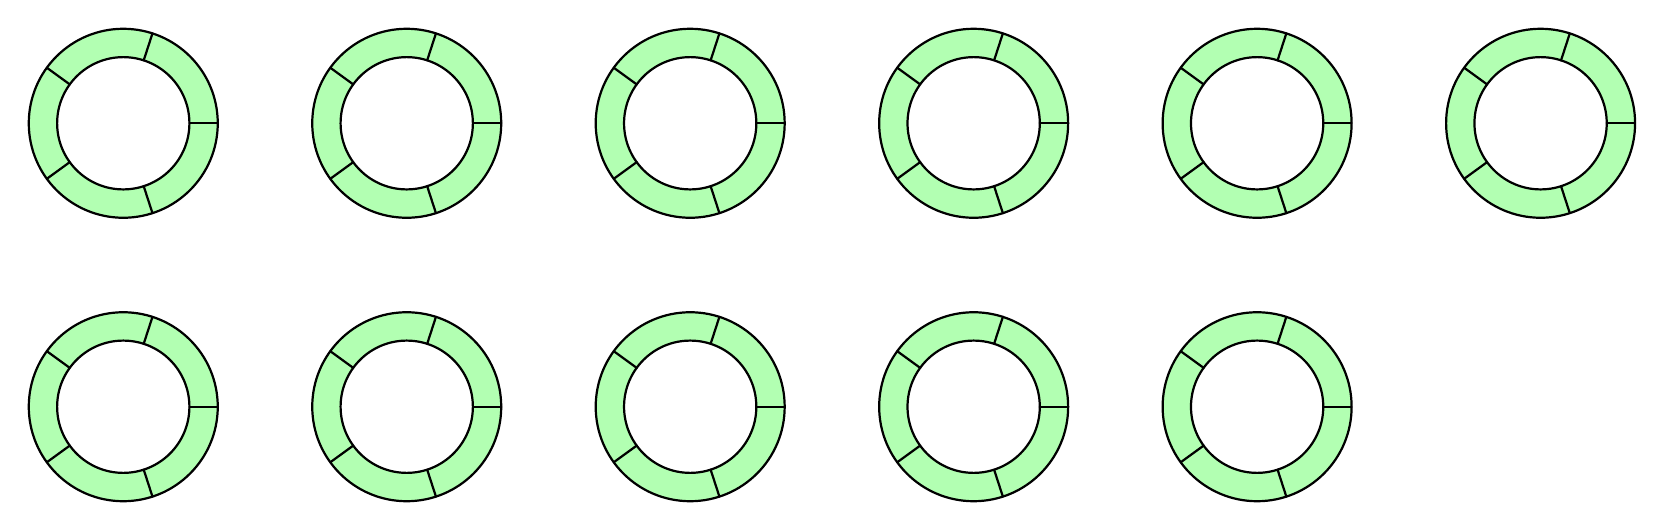
\begin{tikzpicture}[scale=1.2,cap=round,line join=round]
  % We will draw rings of outer radius = 1 and inner radius = 0.7,
  % and put radial lines from 0.7 to 1 except for "skipped" boundaries.

  % A helper command that draws a ring at a given (x,y), then draws
  % all boundaries *except* those in the skip list.
  % Angles we use are 0, 72, 144, 216, 288 (for a total of 5 arcs).

  \def\drawRing#1#2{
    % #1 = the set/list of angles to *skip*
    % #2 = (x,y) shift
    \begin{scope}[shift={#2}]
      % Draw outer green circle and inner white circle to make a 'washer'
      \draw[thick,fill=green!30] (0,0) circle (1);
      \draw[thick,fill=white] (0,0) circle (0.7);

      % Now draw radial lines from radius 0.7 to 1,
      % skipping those angles given in #1.
      \foreach \a in {0,72,144,216,288} {
        % We'll do a little TeX trick: if "\a" is in #1, skip it
        % otherwise draw the boundary:
        \ifx\relax\detokenize{#1}\relax
          % no skip angles at all
          \draw[thick] (\a:0.7) -- (\a:1);
        \else
          % check membership
          \begingroup
            \edef\tmp{\noexpand\ifnum\pdfstrcmp{\detokenize{\a}}{\detokenize{#1}}=1}
          \tmp
            \draw[thick] (\a:0.7) -- (\a:1);
          \fi
          \endgroup
        \fi
      }
    \end{scope}
  }

  % Since we want multiple skips, we can just replicate the scopes
  % manually. For clarity, below we just draw each arrangement with
  % an explicit skip-list and x,y position. 
  % 
  % c5 = 11 tilings. We'll place them in two rows.

  % 1) All singles: no skips
  \drawRing{}{(0,0)}

  % 2) One double + 3 singles.  That double can start at arcs 0..4.
  % Skipping boundary at the shared edge: 72*i
  \drawRing{72}{(3,0)}   % skip boundary at 72
  \drawRing{144}{(6,0)}  % skip boundary at 144
  \drawRing{216}{(9,0)}  % skip boundary at 216
  \drawRing{288}{(12,0)} % skip boundary at 288
  \drawRing{0}{(15,0)}   % skip boundary at 0 => means arcs 4&0 share a 2-tile

  % 3) Two doubles + 1 single.  We skip two boundaries each time.
  % Below are the 5 ways to choose 2 disjoint boundaries to skip:
  % (0,1)-(2,3)-4 => skip 72,216
  % (0,1)-(3,4)-2 => skip 72,288
  % (1,2)-(3,4)-0 => skip 144,288
  % (1,2)-(4,0)-3 => skip 0,144
  % (2,3)-(4,0)-1 => skip 0,216

  \drawRing{72,216}{(0,-3)}    % skip boundaries at 72 and 216
  \drawRing{72,288}{(3,-3)}    % skip 72,288
  \drawRing{144,288}{(6,-3)}   % skip 144,288
  \drawRing{0,144}{(9,-3)}     % skip 0,144
  \drawRing{0,216}{(12,-3)}    % skip 0,216

\end{tikzpicture}



\end{document}
